\newpage
\subsection{Volume Rendering}

Unter dem Begriff Volume Rendering versteht sich eine Reihe von Methoden, die es ermöglichen ein 3D-Datenset zu visualisieren.
Anders als beim Rendern von Geometrien mit einer festen Oberfläche, geht es hierbei darum alle Daten aus
dem jeweiligen Volumen darstellen zu können. Dies sind beispielsweise volumetrische Effekte wie Feuer und Rauch, Wolken oder Nebel,
welche sich, aufgrund ihrer gasförmigen Eigenschaften, nicht wirklich realistisch mit Geometrie darstellen lassen.
Volumen haben keine wirkliche Oberfläche, sondern besteht aus unzähligen winzigen Rußpartikeln.
Möchte man also solche Volumen darstellen, so geraten die bisherigen Herangehensweisen, die sich die Oberflächen der Objekte zunutze machen,
schnell an ihre Grenzen. Beim Grundgedanken des Volume Renderings geht es daher um die Frage, wie das Licht durch diese Volumen
wandert und welchen Einfluss die Partikel darauf haben.
Es gibt einige Faktoren, die beeinflussen was das Auge am Ende von diesem Volumen sieht. Wenn das Licht durch solch ein Volumen wandert
kann es absorbiert, reflektiert oder gestreut werden.
Die Abschwächung durch Streuung und Absorption des Lichtes beim Durchlaufen eines Volumens kann verienfacht mithilfe des Lambert-beerschen Gesetzes wie in \autoref{eqn:beer}
approximiert werden \parencite{Mayerhofer2020}.
Der Absorptionskoeffizient $\sigma_a$ beschreibt dabei die Wahrscheinlichkeit, dass ein Photon auf der Strecke $d$ durch das Medium absorbiert oder anderweitig
reflektiert wird.

\vspace{-0.5cm  }
\begin{equation}
	\label{eqn:beer}
	I_{out} = I_{in} \cdot e^{- ( d \cdot\sigma_a  )}.
\end{equation}





\subsubsection{Ray Marching}

Ray Marching ist eine dieser Möglichkeiten ein Volumen darzustellen. Die Idee hierbei ist es – ähnlich wie beim Ray Tracing –
Strahlen von der Kamera aus durch jeden Pixel des zu rendernden Bildes zu schicken und dabei zu prüfen, ob der Strahl auf etwas trifft.
Der Unterschied besteht hierbei jedoch darin, dass sich Ray Marching auf sogenannten '\textit{signed distance functions}' (SDF) beruht.
SDFs beschreiben, wie weit die nächstgelegene Oberfläche entfernt ist. Befindet sich der Strahl noch außerhalb der Geometrie, so ist
der Wert der Funktion positiv, befindet sich der Strahl innerhalb, so wird der Wert negativ. Dazu wird die Entfernung zu allen Objekten
in der Szene berechnet.

\begin{figure}[h]
	\centering
	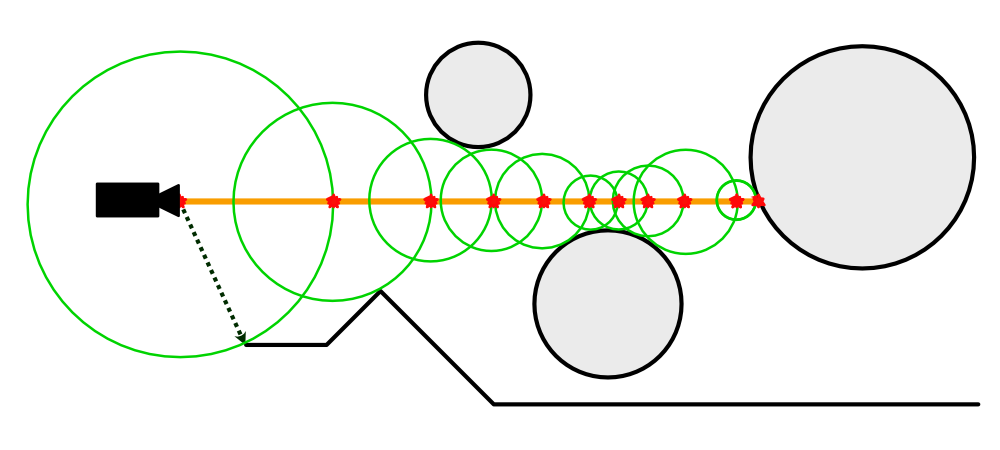
\includegraphics[width=0.80\textwidth]{Grafiken/Basics/Volume/Sphere_Tracing.png}
	\begin{footnotesize}
		\caption{Sphere Tracing: Der Algorithmus wird so lange wiederholt, bis der Radius/Abstand zum nächstgelegenen
			Objekt unter einen bestimmten Grenzwert fällt.}
	\end{footnotesize}
\end{figure}


Im ersten Schritt muss also die Distanz zur nächstgelegenen Oberfläche gefunden werden. Daraus ergibt sich ein Radius in dem sich
mit Sicherheit nichts anderes befindet. Der Strahl bewegt sich nun um die Länge des berechneten Radius' in seine vorgesehene Richtung.
Anschließend werden diese beiden ersten Schritte an der neuen Position wiederholt. Dies passiert so lange, bis die Entfernung gegen einen festgelegten
Grenzwert geht. Dies deutet darauf hin, dass eine Oberfläche getroffen wurde. Diese Variante von Ray Marching wird auch
'\textit{Sphere Tracing}' genannt \parencite{Hart96}. Sphere Tracing ist, im Gegensatz zu einer konstanten Schrittweite, ein effizienter Algorithmus um
Oberflächen entlang des Strahls zu finden, da hiermit die Anzahl der benötigten Schritte deutlich reduziert werden kann.

Jede Oberfläche einer Szene kann durch eine solche Distanzfunktion dargestellt werden.
Eine Kugel lässt sich also beispielsweise durch die folgende Funktion mit ihrer Position in Weltkoordinaten und einem Radius darstellen:

\begin{lstlisting}[language={[Sharp]C}, label={lst:sphereSDF}, caption={SDF einer Kugel im Ursprung},captionpos=b, frame=single]
float sdfSphere( vec3 pos, float radius ){
  return length(pos)-radius;
}
\end{lstlisting}

Mithilfe dieser Funktionen lassen sich mehrere SDFs auf verschiedene Art und Weise kombinieren und neue Formen erzeugen (\autoref{fig:sdfOperators}).
Dabei gibt es Möglichkeiten wie beispielsweise die Vereinigung zweier Objekte, die Schnittmenge oder auch die Differenz.
Mit dem Smooth Union-Operator lassen sich beispielsweise sogenannte Blobs oder Metaballs erzeugen, indem zwischen
den Oberflächen interpoliert wird, sodass diese Geometrien den Anschein erwecken miteinander zu verschmelzen.

\begin{figure}[h]
	\centering
	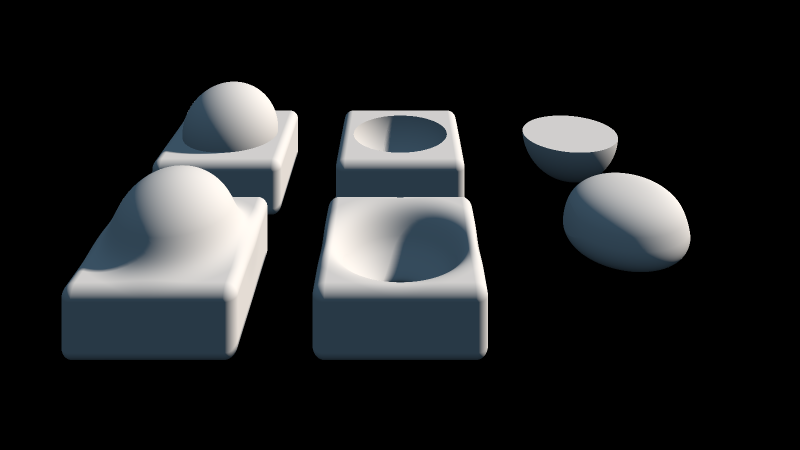
\includegraphics[width=0.80\textwidth]{Grafiken/Basics/Volume/sdfOperators.png}
	\begin{footnotesize}
		\caption{Beispiele von verschiedenen SDF-Operatoren.
			Von links: Union und Smooth Union, Subtraction und Smooth Subtraktion, Intersection und Smooth Intersection}
		\label{fig:sdfOperators}
	\end{footnotesize}
\end{figure}




\subsubsection{Volume Ray Marching}

\begin{figure}[h]
	\centering
	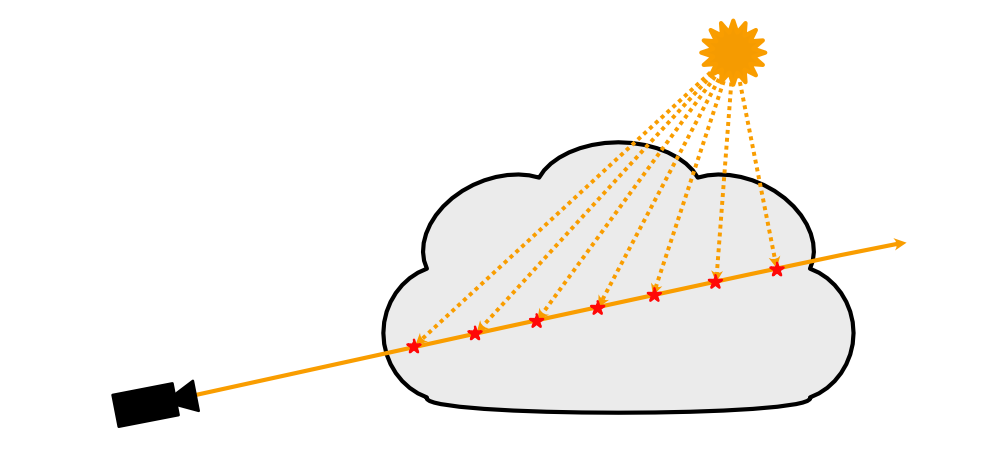
\includegraphics[width=0.80\textwidth]{Grafiken/Basics/Volume/Volume_RayMarching.png}
	\begin{footnotesize}
		\caption{Vereinfachte Darstellung des Volume Ray Marching. Der Weg des Lichtes durch
			das Medium in der Realität aufgrund von In- und Out-Scattering, Absorption oder Emissionen innerhalb des
			Volumens komplexer.}
		\label{fig:volumeRayMarching}
	\end{footnotesize}
\end{figure}


Möchte man nun aber komplexere Volumen darstellen, so gelingt dies mithilfe einer Volumentextur. Der Ansatz bleibt dabei der Gleiche.
Es wird ein Objekt benötigt, welches als eine Domain fungiert. Dieses kann in Form von oben beschriebenen SDFs repräsentiert sein.
Innerhalb dieser Geometrie befindet kann nun alles mögliche dargestellt werden, da hierbei keine Geometrie die Grundlage des
Volumens darstellt. Es lässt sich mittels Code beispielsweise innerhalb eines Würfels eine Kugel darstellen,
sodass es für den Betrachter aussieht wie eine wirkliche Kugel.


Wurde per Sphere Tracing eine Oberfläche ermittelt, so wird in festgelegten Schritten (sample rate) das Innere der Geometrie durchlaufen und an jedem Schritt das
ein Wert berechnet, der sich auch Farbe, Dichte und Tiefe im Volumen berechnet (\autoref{fig:volumeRayMarching}).
Mithilfe von \autoref{eqn:drebin} \parencite{Drebin1988} lässt sich durch das aus einem Voxel austretende Licht ein Farbwert bestimmen. 
Voxel sind das Äquivalent zu einem Pixel im dreidimensionalen Raum und wird durch ein 3D-Gitternetz repräsentiert. 

\begin{equation}
	\label{eqn:drebin}
	C_{out} = C_{in} \cdot (1 - O(x)) + C(x) * O(x).
\end{equation}
<<<Formel stimmt nicht ganz, muss ich noch mal recherchieren>>>


% Ein Nebenprodukt, das sich durch Ray Marching ergibt, ist eine Variante des Ambient Occlusion \parencite{Evans2006}.

